% =====================================================================
% ICLR 2027 submission draft
% 9 pages of content. Appendix unlimited.
%
% Every number is verified against the pipeline. Numbers marked [CI] await
% the bootstrap intervals from the Colab notebook.
% =====================================================================
\documentclass{article}
\usepackage{iclr2027_conference,times}
\usepackage{amsmath,amssymb,booktabs,graphicx,multirow}
\usepackage{float}
\usepackage[utf8]{inputenc}
\usepackage{hyperref}
\usepackage{url}

% Tighten the space around floats. Without this the class stretches
% \textfloatsep to fill the page, leaving a visible gap between a figure or
% table and the text that follows it.
\setlength{\textfloatsep}{12pt plus 2pt minus 2pt}
\setlength{\floatsep}{10pt plus 2pt minus 2pt}
\setlength{\intextsep}{10pt plus 2pt minus 2pt}
\setlength{\dbltextfloatsep}{12pt plus 2pt minus 2pt}

% The class leaves \belowcaptionskip at 0pt, so a caption above a table sits
% flush against the top rule. Give it the same breathing room as above.
\setlength{\belowcaptionskip}{6pt}

% Uncomment ONLY for the camera-ready. While commented, the style file
% anonymises the author block automatically.
%\iclrfinalcopy

\title{HALT: Held-Out-Source Evaluation for
\mbox{Hallucination} Detection in Forensic Video Reporting}

% Authors must not appear in the submitted version; the style file hides
% this block while \iclrfinalcopy is commented out above.
\author{
Author One \\
Affiliation \\
\texttt{email@domain} \\
\And
Author Two \\
Affiliation \\
\texttt{email@domain}
}

\begin{document}
\maketitle

\begin{abstract}
Hallucination detectors for long-form multimodal generation are almost always
evaluated on text from the same source LLMs they were trained on. In forensic
video reporting we show this conflates detection with identifying which LLM
wrote the text. A detector that silently stops working when the underlying
model is updated offers false assurance, in a setting where inventing a detail
and omitting a crime are two different evidentiary failures. We build
\textsc{halt} (Hallucination Across LLMs and Techniques) on a previously
released corpus of 19{,}361 forensic video reports (21.8M words) in which
three frontier multimodal LLMs each describe all 807 surveillance videos,
spanning eleven crime categories, under all eight prompting strategies,
labelled for six hallucination types by a cross-judging panel in which no
model evaluates its own output. Our central result is that
much of what a detector appears to know is the identity of the model that
wrote the report: a predictor reading no report text at all, returning only
the writing model's base rate, captures $70$ to $73\%$ of a detector's
above-chance signal on the fabrication labels against $13\%$ on omission. Withholding a source LLM accordingly costs the fabrication labels $0.104$ to
$0.191$ AUC against $0.035$ to $0.105$ for omission and distortion,
consistently across four detector families from bag-of-words to a fine-tuned
long-context encoder. Two
further findings concern the panel's H1--H6 labels: (i) report length predicts
the panel's scene-fabrication label at AUC $0.727$ but the consensus of two
human annotators who each independently labelled the same 130 reports at only
$0.566$, and (ii) models are not allowed to
judge their own output, so each source LLM is scored by a different pair of
judges; those pairs differ in how often they agree, so comparing hallucination
rates across models partly compares their judges. We release the reliability tiers, the four splits, and
reference implementations of every detector.
\end{abstract}

% =====================================================================
\section{Introduction}

Large language models are increasingly evaluated by other large language
models. Panel-of-judges protocols now label datasets far larger than human
annotation could reach, and those labels underpin leaderboards, safety audits
and deployment decisions. Whether they measure what they are taken to measure is rarely examined, and the
raw verdicts are rarely released.

Hallucination detection inherits both problems. A detector is trained on text
labelled this way and tested on text from the same LLMs that produced the
training set, split at random. Model families differ sharply in surface style
and equally sharply in how often they hallucinate, so a detector with access to
both regularities can score well by recognising which family wrote a passage
and applying its base rate, without assessing whether any claim is supported.
Under a random split this is invisible: the models at test time are the models
at training time.

The distinction matters wherever a detector meets text from a model it has not
seen, which is the normal case. We study it in forensic video reporting and
scope our claims to that domain. There, inventing a detail and omitting a crime
are different evidentiary failures, a screening tool that silently stops
working when the underlying model is updated offers false assurance, and expert
reference annotations written independently of any model are available, which
most long-form generation tasks lack.

Separating the two possibilities requires text from several model families over
identical inputs, labelled per instance, so the source LLM can be withheld while
everything else is fixed. We therefore ask:

\begin{enumerate}\itemsep1pt
\item Do hallucination detectors transfer to source LLMs they were not trained
on, and by how much does performance change?
\item How does detectability depend on hallucination type, and does the type
ordering hold under transfer?
\item Which surface properties carry the detectable signal, and what remains
once source identity is removed?
\item How much of the loss does conditioning on the reference annotation
recover, and for which types?
\item How does panel design shape the labels themselves, both in what drives
judge verdicts and in what excluding self-evaluation implies?
\end{enumerate}

The report corpus, the labelling protocol, the human-validation subset and the
per-judge verdicts are inherited from prior work \citep{priorwork2026}, which
measured how often hallucination occurs and released its materials. Its detectability analysis trained and tested every detector on the same three
source LLMs, so it could not ask whether detection transfers. New here are: the
held-out-source split and the three other video-disjoint partitions that make
the transfer question askable; reference-conditioned detectors and fine-tuned
long-context encoders, so the result cannot be attributed to weak models;
per-type reliability tiers; a length-bias diagnosis scoring the panel and human
labels against the same feature; and a within-judge test showing that excluding self-evaluation confounds the source
LLM with the judges who scored it.

Throughout, we refer to the LLM that produced a report as its \emph{source
LLM}, to distinguish it from the LLMs that later judge it. In the language of
shortcut learning \citep{geirhos2020shortcut}, source identity is a spurious
feature: predictive in distribution, cheaply recoverable from surface style,
and worthless once the source changes.

% =====================================================================
\section{Related Work}

Existing hallucination benchmarks target short outputs and a fixed set of
source LLMs. CHAIR \citep{rohrbach2018object} measures object hallucination in
captions, POPE \citep{li2023evaluating} uses polling, HaluEval
\citep{li2023halueval} benchmarks 35K samples, THRONE \citep{kaul2024throne}
unifies evaluation across six models, Bingo \citep{cui2023holistic} identifies
bias triggers, and VideoHallucer \citep{wang2024videohallucer} extends the
setting to short clips. None varies the writing model while holding the input
fixed, so none can separate a detector that reads evidence from one that reads
style. Detection methods inherit the same limitation: SelfCheckGPT
\citep{manakul2023selfcheckgpt}, semantic entropy \citep{kuhn2023semantic}, and
FActScore \citep{min2023factscore} detect hallucination via consistency,
uncertainty, or fact decomposition, but are evaluated within a single source LLM
or
across several pooled without a held-out condition. Our reference-conditioned
baseline is closest to FActScore, simplified to lexical grounding. The closest
analogue to our argument lies outside the hallucination literature:
\citet{wang2024m4} show that detectors of machine-generated text degrade on
generators they have not seen. That work asks whether text came from a
machine; we ask whether a detector nominally judging content is keyed to the
same signal.

Panel designs \citep{zheng2023judging} and cross-model panels that mitigate
self-preference \citep{panickssery2024llm} are now standard, and their
reliability is typically summarised by a single agreement figure. A growing
body of work questions whether that figure means what it appears to:
\citet{wang2024fair} document position and scoring biases,
\citet{wu2023style} show judges reward stylistic properties over substance,
and \citet{stureborg2024inconsistent} find judges inconsistent across prompts
and biased toward text they find predictable. Length bias sits in this family.
We report reliability per hallucination type against independent human raters,
measure length bias against human labels on the same reports
(Section~\ref{sec:lengthbias}), and show that the no-self-evaluation constraint
itself confounds each source LLM with its judges, which single-figure reporting
hides. Section~\ref{sec:corpus} states what is inherited from prior work and
what is new.

% =====================================================================
% =====================================================================
% Section 3: Methodology. Three subsections.
% Before submitting: replace ANONYMOUS-URL-HERE in the release paragraph.
% =====================================================================

\section{Methodology}
\label{sec:method}

\subsection{Task and corpus}
\label{sec:task}
\label{sec:corpus}

An instance is a triple $(v, m, \tau)$: a surveillance video $v$, a source LLM
$m$, and a prompting strategy $\tau$. The source LLM produces a free-form
forensic report $r$ describing what occurs in $v$, and each report carries an
expert reference annotation $g_v$ written independently of any model. The task
is to predict, from $r$ and optionally $g_v$, six binary labels: H1 scene
fabrication, H5 entity fabrication and H6 phantom actors, which invent content
absent from the footage; H3 crime missed, which drops the criminal act; and H2
crime misclassification and H4 severity minimization, which misstate its nature
or gravity. These group onto three axes, \emph{fabrication}, \emph{omission}
and \emph{distortion}. We report per-type AUC and $F_1$, a macro over the six,
a macro restricted to the reliable types (Section~\ref{sec:labels}), and a
binary any-hallucination score.

\paragraph{Provenance.} The reports, taxonomy, panel protocol, per-judge
verdicts and human-validation subset were introduced and released by
prior work \citep{priorwork2026} to measure hallucination prevalence, and \textsc{halt} reuses all of it as raw material. New here are the
held-out-source formulation of the detection task, the reliability tiering, the
four splits, the reference-conditioned and encoder detectors,
and every analysis in Section~\ref{sec:results}.

The inherited corpus is $19{,}361$ reports on 807 UCF-Crime videos
\citep{sultani2018real} with UCA annotations \citep{yuan2024towards} as
reference, written by three frontier multimodal LLMs under eight prompting
strategies. Two of its properties make the held-out-source question askable.
It is fully crossed up to seven failed API calls, so withholding a source LLM
holds
the input fixed by construction. And verbosity varies by a factor of three under an identical
task, 580 mean words per report for GPT against $1{,}802$ for Gemini, the
regularity Section~\ref{sec:results} shows detectors exploiting.

\begin{figure}[!b]
\centering

\includegraphics[width=\textwidth]{fig_pipeline}
\caption{The \textsc{halt} pipeline. The shaded band is inherited; the
remainder is this paper: aggregating the raw verdicts into labels whose
per-type reliability is calibrated against an independently scored subset,
partitioning the corpus into four video-disjoint splits, and evaluating four
detector families against a base-rate control that reads no report text. In
step 2 each cell is one report, rows are source LLMs and columns are
video-by-strategy conditions; existing benchmarks admit only the standard
split.}
\label{fig:pipeline}
\end{figure}


\subsection{Labels and their reliability}
\label{sec:labels}
\label{sec:protocol}
\label{sec:reliability}

The inherited labels come from a panel of the same three models acting as
judges \citep{zheng2023judging}, each report scored by the two that did not
write it, so self-preference bias \citep{panickssery2024llm} is structurally
excluded \citep{priorwork2026}. Three properties of that design matter
here. It yields two verdicts per report under a conjunctive rule, so
alternative rules can be applied post hoc
(Section~\ref{sec:corpusstats}). Judge inputs cap the reference at $1{,}500$
and the report at $3{,}000$ characters, which
Section~\ref{sec:lengthbias} shows shapes the labels. And no model judging its
own output means each source LLM is scored by a distinct judge pair, the
confound of Section~\ref{sec:confound}.

An inherited subset of 130 reports carries independent labels from two human
annotators, members of the research group rather than forensic practitioners,
who worked from text with the panel's labels hidden. From the rater-rater and
panel-consensus agreements we assign each type a reliability tier and exclude
the low tier from the headline macro; the tiering is ours, and
Section~\ref{sec:corpusstats} reports it.

\subsection{Evaluation setup}
\label{sec:splits}
\label{sec:baselines}
\label{sec:release}


Each video contributes 24 reports, so a split over reports would let a detector
memorise the video rather than learn the phenomenon; Figure~\ref{fig:pipeline}
shows the three partitions.
The standard and held-out-strategy splits are therefore video-disjoint. The
held-out-source split is not, since every video is described by every source
LLM; Section~\ref{sec:inversion} reports a disjointness-enforced variant under
which the effect is larger, so the main tables are conservative.

We provide reference detectors in two families. The first is linear: five
logistic regressions with balanced class weights, differing only in features.
\textbf{Surface} uses verbosity, sentence statistics, hedging density, numeric
detail density, type-token ratio, truncation length, and source and strategy
identity indicators; \textbf{surface-noid} drops the identity features;
\textbf{tfidf} uses word 1--2 gram TF-IDF; \textbf{embed} uses sentence
embeddings; and \textbf{grounded} uses report-versus-reference features only,
namely the rate of report tokens absent from the reference, the rate of
reference tokens absent from the report, Jaccard overlap, reference coverage,
length ratio and TF-IDF cosine. Identity features are dropped automatically on
any split where they are constant in training and unseen at test.

The second family is fine-tuned encoders. One encoder per split, six per-type heads plus a
binary head, report and reference as a sentence pair, positive weights matching
the linear baselines. Context length is chosen rather than defaulted: the judge
saw about 1{,}125 tokens, so a detector at 512 sees less than the judge did. We
report \textbf{DeBERTa-v3-base} at its 512-token limit, \textbf{ModernBERT-base}
at 1{,}280, matching the judge's view, and ModernBERT at 2{,}048, exceeding
it.

The corpus, per-judge verdicts, aggregated labels and rubrics were released
with the prior study. \textsc{halt} adds, and releases: the reliability tiers
with supporting $n$, the four splits, reference implementations of every
detector, and a datasheet \citep{gebru2021datasheets}. The artifact is
available at \url{https://anonymous.4open.science/r/HALT-ANON-7FF2/}.
Supporting tables cited below are in Appendices~\ref{app:strategy}
to~\ref{app:rubrics} of this paper.


% =====================================================================
\section{Results}
\label{sec:results}


\begin{table}[!b]
\caption{Per-type label reliability on the 130-report human-annotated subset.
$\kappa_{\text{panel}}$ compares the panel against the human consensus and is
computed only on reports where the two raters agree; $n$ is that subset size.
Tier thresholds are $\kappa \geq 0.65$ (high) and $\kappa \geq 0.40$ (medium).
H1 is excluded from the headline macro score.}
\label{tab:reliability}
\centering\small
\begin{tabular}{llrrrl}
\toprule
Type & Axis & $n$ & $\kappa_{\text{human-human}}$ & $\kappa_{\text{panel}}$ & Tier \\
\midrule
H1 Scene Fabrication       & Fabrication & 62  & $-0.008$ & 0.150 & low \\
H2 Crime Misclassification & Distortion  & 99  & 0.470 & 0.700 & high \\
H3 Crime Missed            & Omission    & 110 & 0.532 & 0.432 & medium \\
H4 Severity Minimization   & Distortion  & 103 & 0.406 & 0.583 & medium \\
H5 Entity Fabrication      & Fabrication & 64  & 0.082 & 0.811 & high \\
H6 Phantom Actors          & Fabrication & 84  & 0.192 & 0.658 & high \\
\midrule
Macro & & & 0.279 & 0.556 & \\
\bottomrule
\end{tabular}
\end{table}

\subsection{Corpus statistics and label properties}
\label{sec:corpusstats}

The prior study reports $91.1\%$ of reports carrying at least one
hallucination under the released rule. What it does not report is how far that
depends on the rule: a disjunctive rule on the same verdicts gives $98.5\%$ and
$3.55$ per report, a seven-point swing that a release of aggregated labels
alone would conceal.

Reliability is strongly type-dependent (Table~\ref{tab:reliability}): entity
fabrication, misclassification and phantom actors reach $\kappa$ of $0.81$,
$0.70$ and $0.66$ against the human consensus, scene fabrication only $0.15$,
and we exclude it from the headline macro.
Two qualifications apply. The consensus $\kappa$ is computed only where the two
raters agree, a subset of 62 to 110 of 130, so H5's $0.81$ rests on 64 reports and, since the restriction selects the
straightforward cases, $\kappa_{\text{panel}}$ is an upper bound. The raters also agree only modestly
with each other on fabrication (macro $\kappa = 0.28$, $\kappa \approx 0$ on
H1), and the disagreement has a direction: because references are
summary-level, granular detail absent from the summary can be scored as
fabrication. Absolute fabrication prevalence is therefore an upper bound;
relative comparisons are unaffected, since the bias is shared across source
LLMs. Because judge inputs truncate the report at $3{,}000$ characters and the
most verbose source LLMs are the most truncated, truncation can only understate
their fabrication rates.

\subsection{Same-source detection reproduces prior findings}

Under the standard video-disjoint random split we reproduce the prior study's
detectability finding, including that source identity is its most informative
single feature: surface features reach 0.858 on scene fabrication against 0.646
on crime omission, and TF-IDF reaches 0.846 macro and 0.820 binary. That is
what a practitioner would conclude under conventional evaluation.


\begin{figure}[t]
\centering
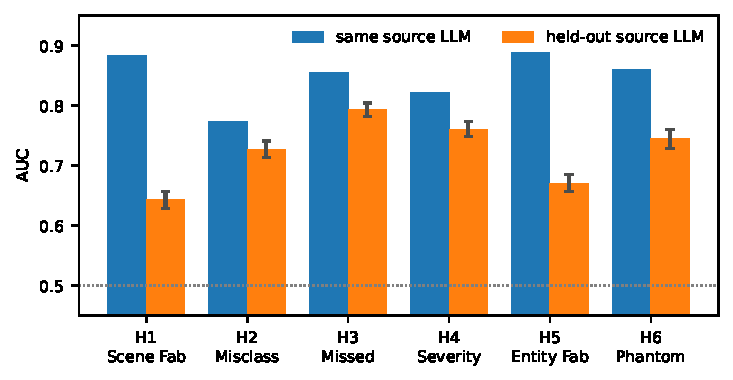
\includegraphics[width=0.62\textwidth]{fig1_inversion}
\caption{Per-type detector AUC (TF-IDF features) under the standard
same-source split and under leave-one-source-out, with bootstrap 95\%
intervals on the held-out bars. The fabrication types (H1, H5) lose roughly
four times as much as the omission and distortion types, inverting the
ordering a same-source evaluation would report.}
\label{fig:inversion}
\end{figure}

\begin{table}[t]
\caption{Degradation from the standard split to leave-one-source-out, by axis,
for four detector families. Drops are LOSO minus standard. The ratio is the
fabrication drop divided by the larger of the omission and distortion drops,
the conservative choice; it is quoted in this form throughout. Fabrication
degrades most in every family.}
\label{tab:families}
\centering\footnotesize
\setlength{\tabcolsep}{4pt}
\begin{tabular}{lrrrrrrr}
\toprule
 & \multicolumn{3}{c}{drop by axis} & & \multicolumn{2}{c}{ANY} & \\
\cmidrule(lr){2-4}\cmidrule(lr){6-7}
Detector & fabr. & omis. & dist. & \textsc{macro} & standard & LOSO & ratio \\
\midrule
tfidf (linear)      & $-$0.191 & $-$0.061 & $-$0.054 & $-$0.123 & 0.820 & 0.566 & 3.1$\times$ \\
DeBERTa-v3, 512     & $-$0.104 & $-$0.035 & $-$0.043 & $-$0.072 & 0.861 & 0.729 & 2.4$\times$ \\
ModernBERT, 1{,}280 & $-$0.163 & $-$0.089 & $-$0.097 & $-$0.129 & 0.833 & 0.644 & 1.7$\times$ \\
ModernBERT, 2{,}048 & $-$0.145 & $-$0.079 & $-$0.105 & $-$0.120 & 0.832 & 0.642 & 1.4$\times$ \\
\bottomrule
\end{tabular}
\end{table}

\subsection{Detection of the fabrication labels degrades most (RQ1--RQ2)}
\label{sec:inversion}

Every detector degrades under leave-one-source-out, and every one degrades
unevenly (Table~\ref{tab:families}, Figure~\ref{fig:inversion}): fabrication
falls by 0.104 to 0.191 AUC against 0.035 to 0.105 for omission and distortion,
a ratio of 1.4 to 3.1. We describe this as degradation of the fabrication
\emph{labels}: the raters agree least on exactly these types
(Section~\ref{sec:corpusstats}), so a property of fabrication and a property of
how fabrication is labelled here cannot be separated. For the lexical detector
the loss inverts the per-type ordering outright, TF-IDF giving fabrication 0.686 against omission 0.793 under
shift having given 0.876 against 0.854 in distribution.

The difference is statistically unambiguous. Bootstrapping the fabrication
degradation minus the omission-and-distortion degradation over 1{,}000
resamples of both splits gives $-0.134$ with a 95\% interval of
$[-0.148, -0.121]$, excluding zero. Per type
(Table~\ref{tab:logoci}): bootstrap 95\% intervals place crime omission above
$0.776$ in every fold, while scene fabrication never exceeds $0.714$ and entity
fabrication never $0.730$, and the intervals do not overlap in any fold.

The effect is not an artifact of residual video overlap: enforcing video
disjointness as well lowers every number and widens the gap, fabrication to
$0.668$ against omission $0.780$ and binary detection to $0.559$
(Appendix~\ref{app:strict}).

For the lexical detector binary detection all but disappears: any-hallucination
AUC falls from 0.820 to 0.566, and on the held-out Claude fold the interval is
$[0.502, 0.578]$, indistinguishable from a coin flip.

Nor is it an artifact of the low-reliability type. Dropping H1 from the
fabrication axis, as the headline macro already does, leaves the ordering
intact: the ratio falls to 2.7, 2.2, 1.5 and 1.1 respectively. Entity
fabrication and phantom actors alone carry the effect.

The encoders retain far more under shift, with binary detection at 0.642 to
0.729 against 0.566, and fabrication remains the worst-hit axis for every one.
The size of the asymmetry does not track detector strength: DeBERTa at 512
tokens is the strongest detector under shift on both binary AUC and macro loss,
yet its ratio of 2.4 exceeds either ModernBERT's. Within the encoder family it
falls as context grows, 2.4 to 1.7 to 1.4, but context does not explain it
either, since TF-IDF sees the whole report untruncated and has the largest
ratio of all. We cannot say whether the ratio plateaus above one. For screening at volume,
the cheapest encoder is thus also the most robust, DeBERTa processing 2.5 times
fewer tokens per report than ModernBERT at 1{,}280.

Context is not the binding constraint. ModernBERT at 1{,}280 tokens sees what
the judge saw, at 2{,}048 it sees more, and the two are indistinguishable under
shift (binary 0.644 against 0.642), consistent with the labels rather than the
detector's input being the limiting factor, though it does not establish that.

Why detectors fail at all is clearer than why fabrication fails most. Scene
fabrication prevalence is $89.6\%$ for Claude and $70.7\%$ for Gemini against
$30.9\%$ for GPT, so recognising the source and applying its base rate scores
well without assessing any claim. Section~\ref{sec:shortcut} measures how
much of the signal that accounts for. Removing
identity features does not help; style is recoverable from the text itself
(Appendix~\ref{app:baselines}).

Transfer also depends on whether a similar failure profile appears in training:
holding out GPT, the only omission-dominant family, drops embedding
scene-fabrication AUC to $0.527$ (Table~\ref{tab:perfold}), while holding out
Claude raises it to
$0.853$.

The held-out-strategy split isolates what is specific to the source LLM rather
than to distribution shift in general. Training on single-turn strategies and
testing on multi-turn ones costs TF-IDF almost nothing: macro 0.846 to 0.837,
binary 0.820 to 0.808 (Appendix~\ref{app:strategy}), and the other feature sets behave the same way. A detector that has never seen multi-turn reports handles
them; one that has never seen a source LLM does not.

\subsection{Source identity is recoverable, and carries most of the signal (RQ3)}
\label{sec:shortcut}

The shortcut can be measured rather than inferred. A TF-IDF classifier
predicting which of the three source LLMs wrote a report reaches $1.000$
accuracy on held-out videos against a chance rate of $0.333$.

What that buys depends sharply on the type (Table~\ref{tab:baserate}). A
predictor with no access to the report, returning only the source LLM's
training-set prevalence, reaches $0.777$ on scene fabrication and $0.773$ on
entity fabrication against the lexical detector's $0.882$ and $0.888$. On the
above-chance scale that is $73\%$ and $70\%$ of what the detector achieves. On
crime omission it reaches $0.545$ against $0.854$, or $13\%$. Detection of the
fabrication labels is therefore mostly source recognition and omission is
mostly not, which is the mechanism behind the transfer asymmetry.

\begin{table}[t]
\caption{How much of a detector's above-chance signal source identity alone
supplies. The base-rate predictor sees no report text: it returns the
training-set prevalence of its label for the source LLM that wrote the report.
Share is $(\text{base-rate}-0.5)/(\text{tfidf}-0.5)$, both on the standard
video-disjoint split.}
\label{tab:baserate}
\centering\small
\begin{tabular}{llrrr}
\toprule
Type & Axis & base rate & tfidf & share \\
\midrule
H1 Scene Fabrication       & fabrication & 0.777 & 0.882 & 73\% \\
H5 Entity Fabrication      & fabrication & 0.773 & 0.888 & 70\% \\
H6 Phantom Actors          & fabrication & 0.662 & 0.859 & 45\% \\
H2 Crime Misclassification & distortion  & 0.595 & 0.773 & 35\% \\
H4 Severity Minimization   & distortion  & 0.599 & 0.822 & 31\% \\
H3 Crime Missed            & omission    & 0.545 & 0.854 & 13\% \\
\midrule
ANY                        & binary      & 0.725 & 0.820 & 70\% \\
\bottomrule
\end{tabular}
\end{table}

\subsection{What grounding buys, and what it does not (RQ4)}
\label{sec:grounding}

Among the linear detectors, reference-conditioned features are the only ones
that move binary detection under shift, reaching 0.702 against 0.566 for TF-IDF
(Appendix~\ref{app:features}), and they give that family's best fabrication axis.
The encoders exceed that without grounding at all: what grounding buys
the linear family, capacity buys the encoder family, and neither removes the
asymmetry of Table~\ref{tab:families}.

One surface cell is diagnostic: on the held-out-Gemini fold severity
minimization falls to $0.443$, below chance, so the relationship learned in distribution reverses on an unseen source
rather than merely weakening, as a shortcut does when its feature is
anti-correlated in the held-out family.

Grounding is, however, worse on omission: 0.577 against TF-IDF's 0.793. Our
grounded features are lexical by construction, so we tested a semantic version: a cross-encoder NLI model scores every report sentence against the
reference and, in the reverse direction, every reference sentence against the
report, aggregated into report-level entailment and contradiction features. The
reverse direction is what should capture a dropped criminal act. It helps
omission and does not rescue it, 0.577 to 0.625 under shift, while costing
elsewhere: the entailment detector reaches 0.632 binary against grounding's
0.702 and 0.648 on omission in distribution against TF-IDF's 0.854. Its
degradation ratio, 4.8, is the largest of any detector we ran. Whether a report
drops the criminal event is therefore not a lexical-representation problem, and
claim-decomposed matching \citep{min2023factscore} may fare no better. No detector wins everywhere, and binary detection under shift
remains the benchmark's open problem, at 0.729 for the strongest detector
against 0.861 in distribution.

\begin{table}[t]
\caption{Does report length predict the panel label or the human label?
AUC of a single feature, report word count, against each label source on the
130-report subset. The human column is restricted to reports where both
raters agree ($n$ from Table~\ref{tab:reliability}). A large positive gap means the feature tracks the judge rather than the
phenomenon. Other features are in Appendix~\ref{app:divergence}.}
\label{tab:artifact}
\centering\footnotesize
\setlength{\tabcolsep}{4pt}
\begin{tabular}{lrrr}
\toprule
Type & AUC vs.\ panel & AUC vs.\ human & Gap \\
\midrule
H1 Scene Fabrication       & 0.727 & 0.566 & $\mathbf{+0.161}$ \\
H4 Severity Minimization   & 0.505 & 0.275 & $\mathbf{+0.230}$ \\
H3 Crime Missed            & 0.484 & 0.390 & $+$0.093 \\
H2 Crime Misclassification & 0.621 & 0.608 & $+$0.013 \\
H5 Entity Fabrication      & 0.784 & 0.800 & $-$0.016 \\
H6 Phantom Actors          & 0.662 & 0.668 & $-$0.006 \\
\bottomrule
\end{tabular}
\end{table}

\subsection{Two properties of the labels themselves (RQ5)}
\label{sec:lengthbias}

Two properties of the labels limit what they can support. The first is a
length bias, exposed by scoring a single feature against both the panel and
the human labels on the shared 130 reports (Table~\ref{tab:artifact}). Report length predicts the panel's
scene-fabrication label at AUC 0.727 but the human label at only 0.566, a gap
of 0.161. Severity minimization diverges more sharply still: for humans, length runs
inverse to the label (0.275), while the panel sees no relationship (0.505).
Entity fabrication and phantom actors show no such gap ($0.784$ versus $0.800$,
$0.662$ versus $0.668$), so the bias is specific rather than pervasive: it says
which labels to distrust, not that all are suspect.

The divergence is specific to verbosity, not to disagreement in general. The
same comparison for the reference-conditioned features gives negative gaps on
almost every type, reaching $-0.236$ on scene fabrication. Only report length
predicts the judge better than it predicts a human reader.

Part of the effect is mechanical. Judge inputs cap at 3{,}000 characters, so
above the cap length is unobservable: the truncation flag alone predicts the
panel's scene-fabrication label at $0.686$, and within truncated reports length
falls to $0.537$. It does not dissolve there. On the 45 untruncated reports the
panel reaches $0.669$ against the human's $0.566$, consistent with the
labelling mechanism of Section~\ref{sec:corpusstats}, where granular detail
absent from a summary-level reference is scored as fabrication. The bias is
real but smaller than the pooled $0.727$ suggests.




\label{sec:confound}
The second property is structural. Excluding self-evaluation has an
unavoidable consequence: each source LLM is scored by a different pair of
judges. Those pairs differ sharply in mutual
agreement. Cohen's $\kappa$ on scene fabrication is $0.850$, $0.415$ and
$0.148$ for the pairs scoring Claude, GPT and Gemini respectively
(Appendix~\ref{app:confound}), so under a conjunctive rule a disagreeing pair
yields fewer positives for purely mechanical reasons. The pairwise agreements
are published with the corpus; what has not been drawn from them is that under
no-self-evaluation they attach to source LLMs rather than to judges. That makes
them a confound between the source LLM and its judges rather than a reliability
statistic, and it follows from the design rather than from this corpus.

The confound is testable because each judge scores exactly two source LLMs,
permitting a within-judge comparison that holds the judge fixed
(Appendix~\ref{app:confound}). Across 18 judge-by-type-by-pair comparisons the ordering
given by the aggregated labels is reproduced in 16, and at the axis level in
all six: every judge that sees GPT calls it omission-dominant, and every judge
that sees Claude or Gemini calls them fabrication-dominant.

Both failures fall on the GPT judge and on fabrication types, where it flags
nearly everything it sees ($92.0\%$ and $96.1\%$ on scene fabrication) and
cannot discriminate. The Claude-versus-Gemini fabrication ordering rests on a 4
to 7 point within-judge margin and is judge-dependent; the two orderings
involving GPT, at 29 to 41 points and reproduced by every judge, are robust.

% =====================================================================
% =====================================================================
\section{Limitations}

\textbf{Three source LLMs.} Leave-one-source-out has three folds, thin
evidence for a claim about model families in general.

\textbf{Fabrication labels, not fabrication.} Our raters agree least on these
types (macro $\kappa = 0.28$) and the panel's label tracks report length where
theirs does not, so a property of fabrication and a property of how it is
labelled here cannot be separated. The asymmetry does survive dropping the
weakest type, in all four detector families.

\textbf{One domain.} The magnitudes should not be assumed to carry to
summarisation, captioning or dialogue; settling that needs a replication on a
second corpus crossed over generators.

\section{Conclusion}

Hallucination detectors are evaluated almost exclusively on text from the
source LLMs they were trained on, and that evaluation cannot distinguish
detecting the phenomenon from recognising the source LLM. In forensic video
reporting the source LLM is trivially recoverable, a base-rate predictor that
reads
no text supplies most of the apparent signal on the fabrication labels, and
withholding a source LLM costs those labels several times what it costs
omission and distortion, consistently across four detector families. The
labels themselves carry a related weakness, tracking report length where human
annotators do not, and the no-self-evaluation constraint that makes the panel
credible also gives each source LLM its own pair of judges. A
held-out-source condition is what separates detection from source recognition,
and per-judge
verdicts are what make the labels auditable.

\section*{Ethics Statement}

The corpus derives from a publicly available surveillance benchmark of
de-identified footage; annotators worked from text only. We release the
resource for auditing and detector development. It is not suitable for
automated legal or investigative decision-making: a system whose error rate
depends on the source LLM, the prompting strategy and the event type does not
meet the standard evidentiary use would require.

\section*{AI Use Statement}

An AI assistant was used to draft and revise sections of this paper from the
authors' direction.


\section*{Reproducibility Statement}

A single entry point rebuilds every label from the released per-judge
verdicts and regenerates every table and figure, verifying the published
corpus statistics on each run so that divergence is caught immediately. All
splits are seeded. Section~\ref{sec:release} lists the released artifacts and
gives the anonymous repository link.

{\setlength{\bibsep}{3pt plus 0.3ex}\small
\bibliography{refs}}
\bibliographystyle{iclr2027_conference}

\appendix
% Appendix pages hold a heading and one or two tables, so \flushbottom
% stretches the slack into the gap under each heading. Let pages end short.
\raggedbottom
\section*{Appendix}

The following material supplements the main text and is referenced from it.
Tables are numbered continuously with the main text.


\section{Held-Out-Strategy Results}
\label{app:strategy}

\begin{table}[H]
\caption{Held-out-strategy split: train on the four single-turn strategies,
test on the four multi-turn ones. Compare the macro column against the standard
split (Table~\ref{tab:noid}) and against leave-one-source-out
(Table~\ref{tab:families}).}
\label{tab:strategy}
\centering\footnotesize
\setlength{\tabcolsep}{4pt}
\begin{tabular}{lrrrrrrrrr}
\toprule
Features & H1 & H2 & H3 & H4 & H5 & H6 & ANY & \textsc{macro} & \textsc{macro-hq} \\
\midrule
surface             & 0.809 & 0.601 & 0.547 & 0.500 & 0.800 & 0.736 & 0.732 & 0.665 & 0.637 \\
surface-noid        & 0.794 & 0.593 & 0.555 & 0.534 & 0.790 & 0.719 & 0.703 & 0.664 & 0.638 \\
tfidf               & 0.868 & 0.753 & 0.859 & 0.832 & 0.873 & 0.839 & 0.808 & 0.837 & 0.831 \\
embed               & 0.745 & 0.681 & 0.617 & 0.730 & 0.632 & 0.624 & 0.633 & 0.671 & 0.657 \\
grounded            & 0.837 & 0.690 & 0.602 & 0.358 & 0.821 & 0.769 & 0.746 & 0.679 & 0.648 \\
\midrule
DeBERTa-v3, 512     & 0.842 & 0.816 & 0.871 & 0.879 & 0.870 & 0.876 & 0.810 & 0.859 & 0.862 \\
ModernBERT, 1{,}280 & 0.826 & 0.777 & 0.844 & 0.863 & 0.857 & 0.873 & 0.787 & 0.840 & 0.843 \\
ModernBERT, 2{,}048 & 0.828 & 0.786 & 0.853 & 0.873 & 0.854 & 0.871 & 0.785 & 0.844 & 0.847 \\
\bottomrule
\end{tabular}
\end{table}

\section{Same-Source Baselines and the Identity Ablation}
\label{app:baselines}

\begin{table}[H]
\caption{Baseline AUC by split for the surface feature families. The
held-out-source rows are the held-out-Gemini fold, not the three-fold mean;
Table~\ref{tab:logoci} gives the per-fold values and means for TF-IDF.
Removing the source and strategy identity indicators (surface-noid) does not
remove the shortcut, because style is recoverable from the text itself: scene
fabrication still reaches 0.811 under the standard split and still collapses to
0.603 on this fold.}
\label{tab:noid}
\centering\footnotesize
\setlength{\tabcolsep}{3pt}
\begin{tabular}{llrrrrrrrr}
\toprule
Features & Split & H1 & H2 & H3 & H4 & H5 & H6 & ANY & \textsc{macro-hq} \\
\midrule
\multirow{3}{*}{surface}
 & random            & 0.858 & 0.690 & 0.646 & 0.653 & 0.865 & 0.772 & 0.765 & 0.725 \\
 & held-out strategy & 0.809 & 0.601 & 0.547 & 0.500 & 0.800 & 0.736 & 0.732 & 0.637 \\
 & held-out src (Gemini) & 0.628 & 0.646 & 0.506 & 0.443 & 0.559 & 0.564 & 0.583 & 0.544 \\
\midrule
\multirow{3}{*}{surface-noid}
 & random            & 0.811 & 0.667 & 0.576 & 0.636 & 0.830 & 0.738 & 0.720 & 0.689 \\
 & held-out strategy & 0.794 & 0.593 & 0.555 & 0.534 & 0.790 & 0.719 & 0.703 & 0.638 \\
 & held-out src (Gemini) & 0.603 & 0.614 & 0.470 & 0.538 & 0.567 & 0.632 & 0.582 & 0.564 \\
\midrule
\multirow{3}{*}{tfidf}
 & random            & 0.882 & 0.773 & 0.854 & 0.822 & 0.888 & 0.859 & 0.820 & 0.839 \\
 & held-out strategy & 0.868 & 0.753 & 0.859 & 0.832 & 0.873 & 0.839 & 0.808 & 0.831 \\
 & held-out src (Gemini) & 0.630 & 0.727 & 0.795 & 0.715 & 0.621 & 0.720 & 0.613 & 0.716 \\
\bottomrule
\end{tabular}
\end{table}

\section{Per-Fold Leave-One-Source-Out}
\label{app:perfold}

\begin{table}[H]
\caption{TF-IDF features, per fold, with bootstrap 95\% confidence intervals
(1{,}000 resamples). The crime-omission interval overlaps neither the scene- nor
the entity-fabrication interval in any fold, which is the separation cited in
Section~\ref{sec:inversion}.}
\label{tab:logoci}
\centering\footnotesize
\setlength{\tabcolsep}{3pt}
\begin{tabular}{lrrrrrrr}
\toprule
Held-out source LLM & H1 & H2 & H3 & H4 & H5 & H6 & ANY \\
\midrule
\multirow{2}{*}{Claude}
 & 0.596 & 0.718 & 0.787 & 0.788 & 0.671 & 0.778 & 0.539 \\
 & \tiny[.581,.611] & \tiny[.704,.732] & \tiny[.776,.799] & \tiny[.774,.801] & \tiny[.658,.686] & \tiny[.765,.788] & \tiny[.502,.578] \\
\multirow{2}{*}{GPT}
 & 0.702 & 0.735 & 0.796 & 0.779 & 0.719 & 0.736 & 0.548 \\
 & \tiny[.689,.714] & \tiny[.719,.749] & \tiny[.785,.807] & \tiny[.767,.790] & \tiny[.707,.730] & \tiny[.713,.760] & \tiny[.531,.566] \\
\multirow{2}{*}{Gemini}
 & 0.630 & 0.727 & 0.795 & 0.715 & 0.621 & 0.720 & 0.613 \\
 & \tiny[.613,.644] & \tiny[.715,.741] & \tiny[.785,.806] & \tiny[.702,.729] & \tiny[.604,.640] & \tiny[.708,.732] & \tiny[.585,.636] \\
\midrule
Mean (held-out)  & 0.643 & 0.727 & 0.793 & 0.761 & 0.671 & 0.744 & 0.566 \\
Random split     & 0.882 & 0.773 & 0.854 & 0.822 & 0.888 & 0.859 & 0.820 \\
Degradation      & $-$0.239 & $-$0.046 & $-$0.061 & $-$0.061 & $-$0.217 & $-$0.115 & $-$0.254 \\
\bottomrule
\end{tabular}
\end{table}

\begin{table}[H]
\caption{AUC on the held-out source LLM, per fold, for every feature set.
Holding out GPT, the only omission-dominant family, drops embedding
scene-fabrication AUC to 0.527 while raising crime-omission AUC to 0.824;
holding out Claude, leaving the similarly fabrication-dominant Gemini, raises
scene fabrication to 0.853.}
\label{tab:perfold}
\centering\footnotesize
\begin{tabular}{llrrrrrrr}
\toprule
Features & Held out & H1 & H2 & H3 & H4 & H5 & H6 & ANY \\
\midrule
\multirow{3}{*}{embed}
 & Claude & 0.853 & 0.659 & 0.689 & 0.674 & 0.862 & 0.661 & 0.670 \\
 & GPT    & 0.527 & 0.624 & 0.824 & 0.716 & 0.566 & 0.673 & 0.587 \\
 & Gemini & 0.671 & 0.627 & 0.645 & 0.644 & 0.655 & 0.560 & 0.528 \\
\midrule
\multirow{3}{*}{grounded}
 & Claude & 0.883 & 0.612 & 0.572 & 0.546 & 0.840 & 0.566 & 0.852 \\
 & GPT    & 0.665 & 0.596 & 0.642 & 0.528 & 0.639 & 0.579 & 0.616 \\
 & Gemini & 0.649 & 0.720 & 0.518 & 0.523 & 0.616 & 0.673 & 0.638 \\
\midrule
\multirow{3}{*}{DeBERTa-v3, 512}
 & Claude & 0.934 & 0.811 & 0.863 & 0.847 & 0.928 & 0.782 & 0.816 \\
 & GPT    & 0.708 & 0.845 & 0.913 & 0.864 & 0.746 & 0.748 & 0.665 \\
 & Gemini & 0.630 & 0.845 & 0.889 & 0.888 & 0.692 & 0.818 & 0.707 \\
\midrule
\multirow{3}{*}{ModernBERT, 1{,}280}
 & Claude & 0.885 & 0.656 & 0.785 & 0.731 & 0.894 & 0.756 & 0.739 \\
 & GPT    & 0.548 & 0.721 & 0.833 & 0.812 & 0.622 & 0.669 & 0.592 \\
 & Gemini & 0.580 & 0.692 & 0.707 & 0.737 & 0.631 & 0.777 & 0.601 \\
\midrule
\multirow{3}{*}{ModernBERT, 2{,}048}
 & Claude & 0.877 & 0.684 & 0.803 & 0.750 & 0.897 & 0.792 & 0.738 \\
 & GPT    & 0.602 & 0.708 & 0.807 & 0.783 & 0.664 & 0.721 & 0.601 \\
 & Gemini & 0.576 & 0.744 & 0.798 & 0.786 & 0.644 & 0.787 & 0.588 \\
\bottomrule
\end{tabular}
\end{table}

\section{Video-Disjoint Leave-One-Source-Out}
\label{app:strict}

Holding out a source LLM leaves the same videos on both sides of the split,
since every video is described by every source LLM. Re-running the three folds
with video disjointness additionally enforced (training on 9{,}003 reports,
testing on 1{,}016) lowers every number and widens the gap: the fabrication
axis falls to 0.668 and omission to 0.780, so the omission-minus-fabrication
margin grows from 0.107 to 0.112, and binary detection falls to 0.559. The
figures in the main text are therefore the conservative ones.

\section{The Judge-Pair Confound}
\label{app:confound}

\begin{table}[H]
\caption{Judge-pair agreement and within-judge axis rates. The pairs differ by
a factor of five on the fabrication types; the within-judge rates hold the
judge fixed, and the dominant axis is reproduced by every judge for every
source LLM it sees.}
\label{tab:confound}
\centering\footnotesize
\begin{tabular}{llrrr}
\toprule
\multicolumn{5}{l}{\textbf{(a) Pair agreement, Cohen's $\kappa$}} \\
Source LLM & Judged by & H1 & H5 & overall \\
\midrule
Claude & GPT + Gemini    & 0.850 & 0.845 & 0.809 \\
GPT    & Claude + Gemini & 0.415 & 0.475 & 0.580 \\
Gemini & Claude + GPT    & 0.148 & 0.138 & 0.614 \\
\bottomrule
\end{tabular}

\vspace{1em}

\begin{tabular}{llrrrl}
\toprule
\multicolumn{6}{l}{\textbf{(b) Within-judge axis rates (\%)}} \\
Judge & Source LLM & Fabrication & Omission & Distortion & Dominant \\
\midrule
Claude & GPT    & 28.6 & 55.7 & 42.7 & omission \\
Claude & Gemini & 66.7 & 54.3 & 39.8 & fabrication \\
GPT    & Claude & 77.8 & 41.7 & 36.0 & fabrication \\
GPT    & Gemini & 79.2 & 49.4 & 38.1 & fabrication \\
Gemini & Claude & 72.7 & 44.5 & 26.8 & fabrication \\
Gemini & GPT    & 44.1 & 53.1 & 33.1 & omission \\
\bottomrule
\end{tabular}
\end{table}

\section{Label-Source Divergence, All Features}
\label{app:divergence}

\begin{table}[H]
\caption{AUC of each single feature against the panel label and against the
human label, on the 130-report subset. Table~\ref{tab:artifact} reports the
report-length column. Every reference-conditioned feature diverges in the
opposite direction: on grounded quantities the panel does not diverge from the
human raters.}
\label{tab:divergencefull}
\centering\footnotesize
\begin{tabular}{lrrrrrr}
\toprule
Type & \multicolumn{2}{c}{novel rate} & \multicolumn{2}{c}{missing rate} & \multicolumn{2}{c}{hedging rate} \\
\cmidrule(lr){2-3}\cmidrule(lr){4-5}\cmidrule(lr){6-7}
 & panel & human & panel & human & panel & human \\
\midrule
H1 Scene Fabrication       & 0.535 & 0.546 & 0.300 & 0.536 & 0.551 & 0.451 \\
H2 Crime Misclassification & 0.545 & 0.600 & 0.500 & 0.565 & 0.471 & 0.573 \\
H3 Crime Missed            & 0.618 & 0.644 & 0.671 & 0.692 & 0.522 & 0.547 \\
H4 Severity Minimization   & 0.547 & 0.661 & 0.608 & 0.730 & 0.616 & 0.636 \\
H5 Entity Fabrication      & 0.467 & 0.595 & 0.254 & 0.342 & 0.464 & 0.577 \\
H6 Phantom Actors          & 0.567 & 0.607 & 0.408 & 0.450 & 0.461 & 0.450 \\
\bottomrule
\end{tabular}
\end{table}

\section{Feature Sets Under Leave-One-Source-Out}
\label{app:features}

\begin{table}[H]
\caption{Feature sets and encoders under leave-one-source-out, averaged over
the three folds. Axis scores are the mean per-type AUC within the axis. Among
the linear detectors, reference-conditioned features are the only ones that
recover binary detection; the fine-tuned encoders exceed them without
grounding.}
\label{tab:grounded}
\centering\small
\begin{tabular}{lrrrrr}
\toprule
Features & Fabrication & Omission & Distortion & \textsc{macro} & ANY \\
\midrule
surface             & 0.584 & 0.506 & 0.545 & 0.558 & 0.583 \\
nli-grounded        & 0.599 & 0.625 & 0.526 & 0.579 & 0.632 \\
embed               & 0.670 & 0.719 & 0.657 & 0.674 & 0.595 \\
tfidf               & 0.686 & 0.793 & 0.744 & 0.723 & 0.566 \\
grounded            & 0.679 & 0.577 & 0.587 & 0.631 & 0.702 \\
grounded+surface    & 0.691 & 0.607 & 0.599 & 0.646 & 0.652 \\
\midrule
DeBERTa-v3, 512     & \textbf{0.776} & \textbf{0.888} & \textbf{0.850} & \textbf{0.820} & \textbf{0.729} \\
ModernBERT, 1{,}280 & 0.707 & 0.775 & 0.725 & 0.724 & 0.644 \\
ModernBERT, 2{,}048 & 0.729 & 0.803 & 0.742 & 0.746 & 0.642 \\
\bottomrule
\end{tabular}
\end{table}

\section{Rubrics and Full Corpus Statistics}
\label{app:rubrics}

The verbatim judge rubric, the human-rater instructions, the per-cell
hallucination rates for all 24 source-LLM-by-strategy combinations, and the
datasheet are in the released artifact, which also regenerates every table
above from the raw per-judge verdicts.


\end{document}
